\section{رویکرد دوم: معیارهای فرآیند مبتنی بر جهش}
همانطور که در قسمت \ref{sec:method-phase-two} اشاره شده چهار معیار معرفی شدند و مبتنی بر جهش نامیده شدند. این قسمت به نحوه‌ی پیاده‌سازی دسته‌ی دوم از معیارها را شرح خواهد داد. 
\begin{itemize}
\item
\متن‌سیاه{تعداد جهش‌یافته‌های تولید شده‌ی جدید نسبت به انتشار قبلی برنامه:}
به منظور محاسبه‌ی این معیار ابتدا لازم است که مشخص شود که پرونده‌ی مورد نظر نسبت به انتشار قبلی چه تغییراتی داشته است. این کار با استفاده از ابزار JGit انجام  می‌شود. JGit این امکان را فراهم می‌کند که دو پرونده در دو ثبت متفاوت مقایسه شوند و مشخص می‌کند که کدام خطوط حذف شده‌اند و کدام خطوط اضافه شده‌اند. در اینجا لازم است خطوط اضافه شده  مشخص شود. سپس با استفاده از ابزار Major جهش‌یافته‌ها تولید می‌شود. در  قسمت  \ref{sec:tools-major} توضیح داده شد که پس تولید جهش‌یافته‌ها یک فایل خروجی نیز به نام mutant.log تولید می‌شود که در آن مشخص شده در هر خط از برنامه چه جهش‌یافته‌هایی تولید شده است. حال کافیست تعداد جهش‌یافته‌های تولید شده در خطوطی شمرده شوند که ابزار Jgit آن‌ها را به عنوان خطوط جدید نسبت به انتشار قبلی معرفی کرده است. بدین ترتیب این معیار محاسبه خواهد شد.\\
لازم به ذکر است روش یاد شده پایه‌ی محاسبه‌ی معیار بعدی و معیارهای رویکرد سوم است.
\item
\متن‌سیاه{تعداد جهش‌یافته‌های متمایز در چند انتشار اخیر:}

 به منظور افزایش کارایی ابتدا بررسی می‌شود که فایل مورد نظر در آن انتشار وجود دارد یا خیر در صورت عدم وجود محاسبات برای آن انتشار انجام نمی‌گیرد.
برای محاسبه ابتدا چهار انتشار قبلی  با استفاده از پرسمان  \ref{code:previous-releases} از جدول ProjectRelease بازیابی می‌شود. سپس مشابه معیار قبلی جهش‌یافته‌های جدید نسبت به انتشار قبلی برای هر انتشار محاسبه می‌شود و با هم جمع زده می‌شود.  یک جدول برای نتایج تولید جهش‌یافته‌ها  به نام  DistinctMutantLog در نظر گرفته شده که تعداد جهش‌یافته‌های جدید برای هر انتشار نسبت به انتشار قبلی در آن ذخیره می‌گردد. از مزایای ایجاد این جدول پایداری در انجام محاسبات است به عنوان مثال  در صورت توقف محاسبات امکان از سرگیری محاسبات از محل توقف وجود  دارد و همچنین  با نگهداری به عنوان یک مجموعه داده می‌تواند در پژوهش‌های دیگر به کار گرفته شود. نمایی از جدول در شکل زیر آمده است. به طور مثال سطر اول جدول بیان می‌کند که در انتشاری از برنامه با شماره ثبت  \lr{..21a}  پرونده‌ی شماره یک شماره یک از فایلهای حاوی خطا 430 جهش‌یافته‌ی جدید نسبت به انتشار قبلی داشته است.
\begin{latin}
	\begin{lstlisting}[language=SQL]
SELECT * FROM ProjectRelease WHERE Project = :project AND
 SequenceNumber <  
	(SELECT SequenceNumber FROM ProjectRelease WHERE 
	 Project = :project AND CommitId = :releaseCommit) 
 ORDER BY SequenceNumber DESC LIMIT 4 
\end{lstlisting}
\end{latin}
\captionof{lstlisting}{بازیابی چهار نسخه‌ی اخیر یک ثبت}
\label{code:previous-releases}

\begin{figure}[H]
	\centering
	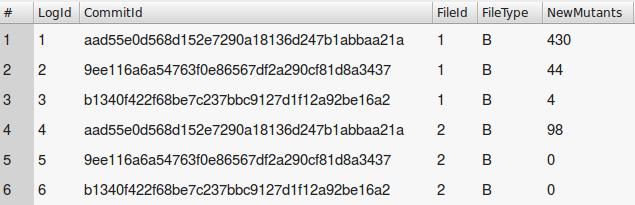
\includegraphics[width=1\textwidth]{img/case_study/distinct-mutant-log.png}
	\caption{نمایی از جدول تعداد جهش‌یافته‌های متمایز در انتشارها}
	\label{fig:distinct-mutant-log}
\end{figure}
\item
\متن‌سیاه{میزان تغییرات مثبت امتیاز جهش  در چند انتشار اخیر:}
ابتدا انتشارها  مشابه معیار قبلی بازیابی می‌شوند و سپس برای هر یک تحلیل جهش انجام می‌گردد. نتایج جهش در جدولی به نام ReleaseMutation قرار می‌گیرد.  نمایی از این جدول در شکل  \ref{fig:release-mutation} آمده است. سپس هر انتشار با انتشار قبلی مقایسه می‌شود و در صورتی که تغییر امتیاز جهش  مثبت باشد با مجموعه تغییرات مثبت جمع می‌گردد. 
\begin{figure}[H]
	\centering
	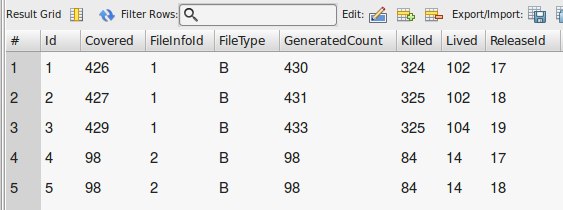
\includegraphics[width=1\textwidth]{img/case_study/release-mutation.png}
	\caption{نمایی از جدول نتایج تحلیل جهش در انتشارها}
	\label{fig:release-mutation}
\end{figure}
\item
\متن‌سیاه{میزان تغییرات منفی امتیاز جهش  در چند انتشار اخیر:}
به طور مشابه با معیار قبلی عمل می‌گردد با این تفاوت که تغییرات منفی در نظر گرفته می‌شود. 
\end{itemize}
